\documentclass[10pt]{beamer}
\usepackage{appendixnumberbeamer}
\usepackage{booktabs}
\usepackage[scale=2]{ccicons}
\usepackage{pgfplots}
\usepackage{xspace}
\usepackage{xcolor}
\usepackage{caption}

\usetheme[progressbar=frametitle]{metropolis}
\usepgfplotslibrary{dateplot}
\newcommand{\themename}{\textbf{\textsc{metropolis}}\xspace}
\captionsetup[figure]{labelformat=empty}

% ---------------------------------------------------------
\title{Artificial astrocyte networks}
% \subtitle{A modern beamer theme}
% \date{\today}
\date{}
\author{Erik J Peterson}
\institute{CoAxLab\\Carnegie Mellon University}

% ---------------------------------------------------------
\begin{document}
\maketitle

\begin{frame}{Table of contents.}
  \setbeamertemplate{section in toc}[sections numbered]
  \tableofcontents%[hideallsubsections]
\end{frame}

% ---------------------------------------------------------
\section[]{Goal.}
\begin{frame}[fragile]{Goal}
\begin{itemize}
    \item Use models and proof methods from artificial intelligence to try and set an \alert{upper bound} on astrocyte computation.
\end{itemize}
\end{frame}

% ---------------------------------------------------------
\section[ANNs]{What are artificial neural networks?}
\begin{frame}[fragile]{What are ANNs?}
\begin{itemize}
\item By example.
\item Sparse networks.
\end{itemize}
\end{frame}

\begin{frame}[fragile]{Classic example: visual digit recognition.}
\begin{columns}
\column{0.5\textwidth}
\centering
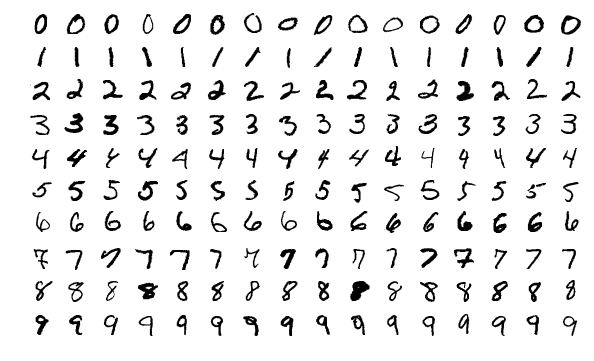
\includegraphics[scale=0.25]{images/minst.png}
\column{0.5\textwidth}
\centering
 = 1,2,3,4,5,6,\ldots
\end{columns}
\end{frame}

\begin{frame}[fragile]{Nine recognition.}
\begin{columns}
\column{0.5\textwidth}
\begin{figure}
    \centering
    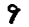
\includegraphics[scale=4]{images/nine.png} 
\end{figure}
\column{0.5\textwidth}
\centering
 $= 9$
\end{columns}
\end{frame}

\begin{frame}[fragile]{Digit recognition.}
\begin{columns}
\column{0.5\textwidth}
\begin{figure}
    \centering
    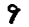
\includegraphics[scale=4]{images/ninepixeled.png} 
\end{figure}
\column{0.5\textwidth}
\centering
 $ $
\end{columns}
\end{frame}

\begin{frame}[fragile]{Digit recognition.}
\begin{columns}
\column{0.5\textwidth}
\begin{figure}
    \centering
    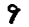
\includegraphics[scale=4]{images/nine.png} 
    \caption{\textbf{x}}
\end{figure}
\column{0.5\textwidth}
\centering
 $= 9$
\end{columns}
\end{frame}

\begin{frame}[fragile]{Digit recognition.}
\begin{columns}
\column{0.5\textwidth}
\centering
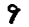
\includegraphics[scale=2]{images/nine.png} 
\column{0.5\textwidth}
\centering
 $\sum x_{ij} = 9$
\end{columns}
\end{frame}

% ---------------------------------------------------------
\section[AANs]{Defining artificial astrocyte networks.}

\begin{frame}[fragile]{Basic astrocyte properties}
\begin{itemize}
    \item $[Ca^{2+}]$ dynamics
    \item Glia transmission
\end{itemize}
\end{frame}

\begin{frame}[fragile]{Assumption 1.}
\begin{itemize}
    \item $[Ca^{2+}]$ dynamics $\leftrightarrow$ firing rate
\end{itemize}
\end{frame}

\begin{frame}[fragile]{Basic astrocyte limits.}
\begin{itemize}
    \item No synapses
    \item No axons 
\end{itemize}
\end{frame}

\begin{frame}[fragile]{Basic astrocyte limits.}
\begin{itemize}
    \item No $w_i$
    \item No $\sum$
\end{itemize}
\end{frame}

\begin{frame}[fragile]{Assumption 2 ($w_i$).}
\begin{itemize}
    \item Learned $[Ca^{2+}]$-dependent release
    \item Directional
\end{itemize}
\end{frame}
\begin{frame}[fragile]{Assumption 3 ($\sum$).}
\begin{itemize}
    \item Directional $[Ca^{2+}]$ waves
\end{itemize}
\end{frame}

% ---------------------------------------------------------
\section[In theory.]{Theory.}
\begin{frame}[fragile]{Computational calcium waves.}
\begin{itemize}
\item Let's study a forward moving $[Ca^{2+}]$ wave.
\item (With Assumptions 1-3)
\item \alert{Prove}: it is a universal function approximator.
\end{itemize}
\end{frame}

\begin{frame}[fragile]{A universal function approximator?}
$|F(x) - f(x)| < \epsilon$
\end{frame}

\begin{frame}[fragile]{Proof sketch.}
\begin{itemize}
\item Astrocyte Sudoku
\end{itemize}
\end{frame}

% ---------------------------------------------------------
\section[In practice.]{Practice.}
\begin{frame}[fragile]{Astrocyte layers.}
\begin{itemize}
    \item Spread
    \item Gather
    \item Slide
\end{itemize}
\end{frame}

\begin{frame}[fragile]{A fundamental limit?}
\begin{itemize}
\item Width requires depth.
\end{itemize}
\end{frame}

\begin{frame}[fragile]{Results.}
\begin{figure}
    \centering
    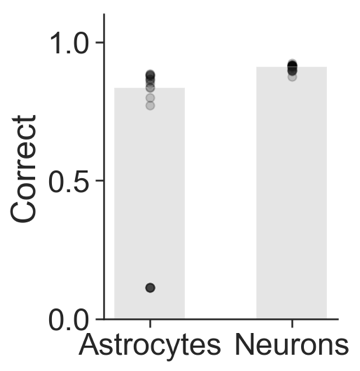
\includegraphics[scale=0.5]{images/results.png} 
    % \caption{Classification accuracy.}
\end{figure}
\end{frame}

\begin{frame}[fragile]{Conclusions.}
\begin{itemize}
\item AANs $\rightarrow$ universal function approximator.
\item AANs can solve hard vision problems.
\item An \alert{upper bound} for the performance of real astrocytes? 
\end{itemize}
\end{frame}

\begin{frame}[fragile]{Open science.}
\begin{itemize}
\item[Code] \url{github.com/CoAxLab/glia_playing_atari}
\item[Talk] \url{github.com/parenthetical-e/glia-talk-sfn-2019}
\item[] 
\item[] \alert{Thank you!}
\end{itemize}
\end{frame}


% ---------------------------------------------------------
% \begin{frame}[allowframebreaks]{References}
%   \bibliography{demo}
%   \bibliographystyle{abbrv}
% \end{frame}

% ---------------------------------------------------------
\end{document}
